%!TEX program = xelatex
\documentclass[11pt]{beamer}

\usepackage{amsfonts}
\usepackage{amsmath}
\usepackage{blindtext}
\usepackage{enumitem}

\usetheme{SaoPaulo}

\title{Python Basics!}
\subtitle{multidimensional indexing, file operations}
\author{CS101 Lecture \#10}
\date{2016-09-26}

\setcounter{showSlideNumbers}{1}

\begin{document}
  \setcounter{showProgressBar}{0}
  \setcounter{showSlideNumbers}{0}

%%%%%%%%%%%%%%%%%%%%%%%%%%%%%%%%%%%%%%%%%%%%%%%%%%%%%%%%%%%%%%%%%%%%%%%%%%%%%%%%
\frame{\titlepage}

%%%%%%%%%%%%%%%%%%%%%%%%%%%%%%%%%%%%%%%%%%%%%%%%%%%%%%%%%%%%%%%%%%%%%%%%%%%%%%%%
\setcounter{framenumber}{0}
\setcounter{showProgressBar}{1}
\setcounter{showSlideNumbers}{1}

%%%%%%%%%%%%%%%%%%%%%%%%%%%%%%%%%%%%%%%%%%%%%%%%%%%%%%%%%%%%%%%%%%%%%%%%%%%%%%%%
\section{Administrivia}

%%%%%%%%%%%%%%%%%%%%%%%%%%%%%%%%%%%%%%%%%%%%%%%%%%%%%%%%%%%%%%%%%%%%%%%%%%%%%%%%
\begin{frame}
  \frametitle{Administrivia}
  \Enlarge
  \begin{itemize}
  \myitem  Homework \#5 is due Friday Sep.\ 30.
  \myitem  Midterm \#1 will be Monday Oct.\ 3.  (evening) \\ \textcolor{CS101GradBot}{No class on Monday, \\ Labs WILL be held all week.}
  \end{itemize}
\end{frame}

%%%%%%%%%%%%%%%%%%%%%%%%%%%%%%%%%%%%%%%%%%%%%%%%%%%%%%%%%%%%%%%%%%%%%%%%%%%%%%%%
\section{Warmup Quiz}

%%%%%%%%%%%%%%%%%%%%%%%%%%%%%%%%%%%%%%%%%%%%%%%%%%%%%%%%%%%%%%%%%%%%%%%%%%%%%%%%
\begin{frame}[fragile]
  \frametitle{Question \#1}
  \Enlarge

  \begin{semiverbatim}
t = ''
for c in s:
    if c not in 'aeiou':
        t += c
  \end{semiverbatim}
  What does this program do to string \texttt{s}?
  \begin{enumerate}[label=\Alph*]
  \item  Counts the vowels.
  \item  Removes the vowels.
  \item  Counts the consonants.
  \item  Removes the consonants.
  \end{enumerate}
\end{frame}

%%%%%%%%%%%%%%%%%%%%%%%%%%%%%%%%%%%%%%%%%%%%%%%%%%%%%%%%%%%%%%%%%%%%%%%%%%%%%%%%
\begin{frame}[fragile]
\frametitle{Question \#2}
\Enlarge

\begin{semiverbatim}
x = 0
for i in [ 1,4950,99,100 ][ 0:-1 ]:
    x = i
\end{semiverbatim}
  What is the final value of \texttt{x}?
  \begin{enumerate}[label=\Alph*]
  \item  \texttt{0}
  \item  \texttt{99}
  \item  \texttt{100}
  \item  \texttt{4950}
  \end{enumerate}
\end{frame}

%%%%%%%%%%%%%%%%%%%%%%%%%%%%%%%%%%%%%%%%%%%%%%%%%%%%%%%%%%%%%%%%%%%%%%%%%%%%%%%%
\section{Multidimensional Indexing}

%%%%%%%%%%%%%%%%%%%%%%%%%%%%%%%%%%%%%%%%%%%%%%%%%%%%%%%%%%%%%%%%%%%%%%%%%%%%%%%%
\begin{frame}[fragile]
  \frametitle{Nested \texttt{list}s}
  \Enlarge

  \begin{itemize}
  \myitem  Just as we can nest control structures, we can nest container values.
  \end{itemize}
  \begin{semiverbatim}
a = [ [ 1, 2 ], [ 3, 4 ] ]
  \end{semiverbatim}
  \begin{itemize}
  \myitem  What does this look like?
  \end{itemize}
\end{frame}

%%%%%%%%%%%%%%%%%%%%%%%%%%%%%%%%%%%%%%%%%%%%%%%%%%%%%%%%%%%%%%%%%%%%%%%%%%%%%%%%
\begin{frame}[fragile]
  \frametitle{Multidimensional indexing}
  \Enlarge

  \begin{itemize}
  \myitem  Access member values of a nested container by coordinates:
  \end{itemize}
  \begin{semiverbatim}
a = [ [ 1, 2 ], [ 3, 4 ] ]
a[0]    #?
a[0][0] #?
  \end{semiverbatim}
  \begin{itemize}
  \myitem  Python orders by \texttt{(row, column)}---that is, the first number selects the row and the second selects the column in that row.
  \myitem  \textcolor{red}{Side effect:  easy to select rows, hard to select columns!}
  \end{itemize}
\end{frame}

%%%%%%%%%%%%%%%%%%%%%%%%%%%%%%%%%%%%%%%%%%%%%%%%%%%%%%%%%%%%%%%%%%%%%%%%%%%%%%%%
\begin{frame}[fragile]
  \frametitle{Example}
  \Enlarge

  \begin{semiverbatim}
a = [ [1,2,3], [4,5,6], [7,8,9] ]
  \end{semiverbatim}
  How would you refer to the value 6?
  \begin{enumerate}[label=\Alph*]
  \item  \texttt{a[2][3]}
  \item  \texttt{a[1][2]}
  \item  \texttt{a[2,3]}
  \item  \texttt{a[2][1]}
  \end{enumerate}
\end{frame}

%%%%%%%%%%%%%%%%%%%%%%%%%%%%%%%%%%%%%%%%%%%%%%%%%%%%%%%%%%%%%%%%%%%%%%%%%%%%%%%%
\begin{frame}[fragile]
  \frametitle{Container methods}
  \Enlarge

  \begin{itemize}
  \myitem  What is the difference between \texttt{list.extend} and \texttt{list.append}?
  \end{itemize}
  \begin{semiverbatim}
a = [ 1, 2 ]
b = [ 3, 4 ]
c = a.extend(b)  #?
d = a.append(b)  #?
  \end{semiverbatim}
\end{frame}

%%%%%%%%%%%%%%%%%%%%%%%%%%%%%%%%%%%%%%%%%%%%%%%%%%%%%%%%%%%%%%%%%%%%%%%%%%%%%%%%
\section{File Operations}

%%%%%%%%%%%%%%%%%%%%%%%%%%%%%%%%%%%%%%%%%%%%%%%%%%%%%%%%%%%%%%%%%%%%%%%%%%%%%%%%
\begin{frame}[fragile]
  \frametitle{Files}
  \Enlarge

  \begin{itemize}
  \myitem  It is uncommon to generate the source data in the same program as one uses it.
  \myitem  What is a file?
  \end{itemize}
\end{frame}

%%%%%%%%%%%%%%%%%%%%%%%%%%%%%%%%%%%%%%%%%%%%%%%%%%%%%%%%%%%%%%%%%%%%%%%%%%%%%%%%
\begin{frame}[fragile]
  \frametitle{Punch card}

  \includegraphics[width=\textwidth]{./img/file-structure-card.png}
\end{frame}

% http://homepage.cs.uiowa.edu/~jones/cards/collection/i-program.html

%%%%%%%%%%%%%%%%%%%%%%%%%%%%%%%%%%%%%%%%%%%%%%%%%%%%%%%%%%%%%%%%%%%%%%%%%%%%%%%%
\begin{frame}[fragile]
  \frametitle{Punch card deck---5 MB}

  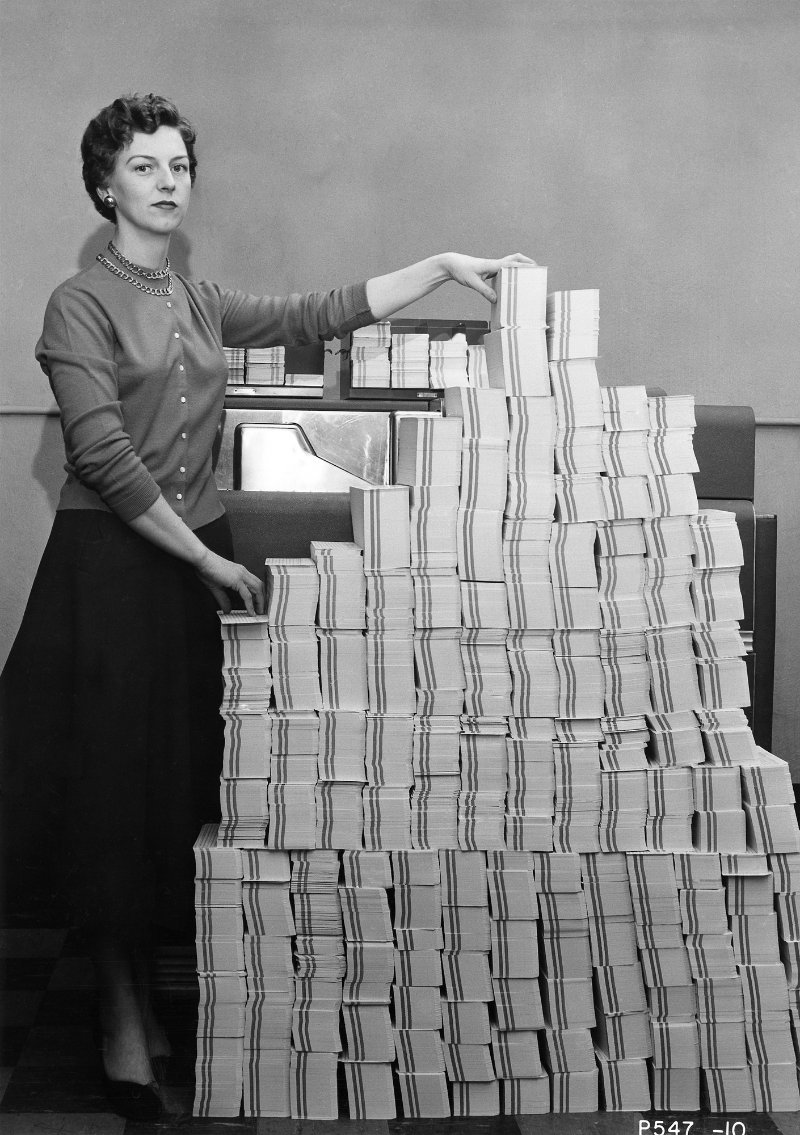
\includegraphics[height=0.75\textheight]{./img/file-structure-deck.png}
\end{frame}

% http://www.computerhistory.org/revolution/memory-storage/8/326

%%%%%%%%%%%%%%%%%%%%%%%%%%%%%%%%%%%%%%%%%%%%%%%%%%%%%%%%%%%%%%%%%%%%%%%%%%%%%%%%
\begin{frame}[fragile]
  \frametitle{Secondary storage}

  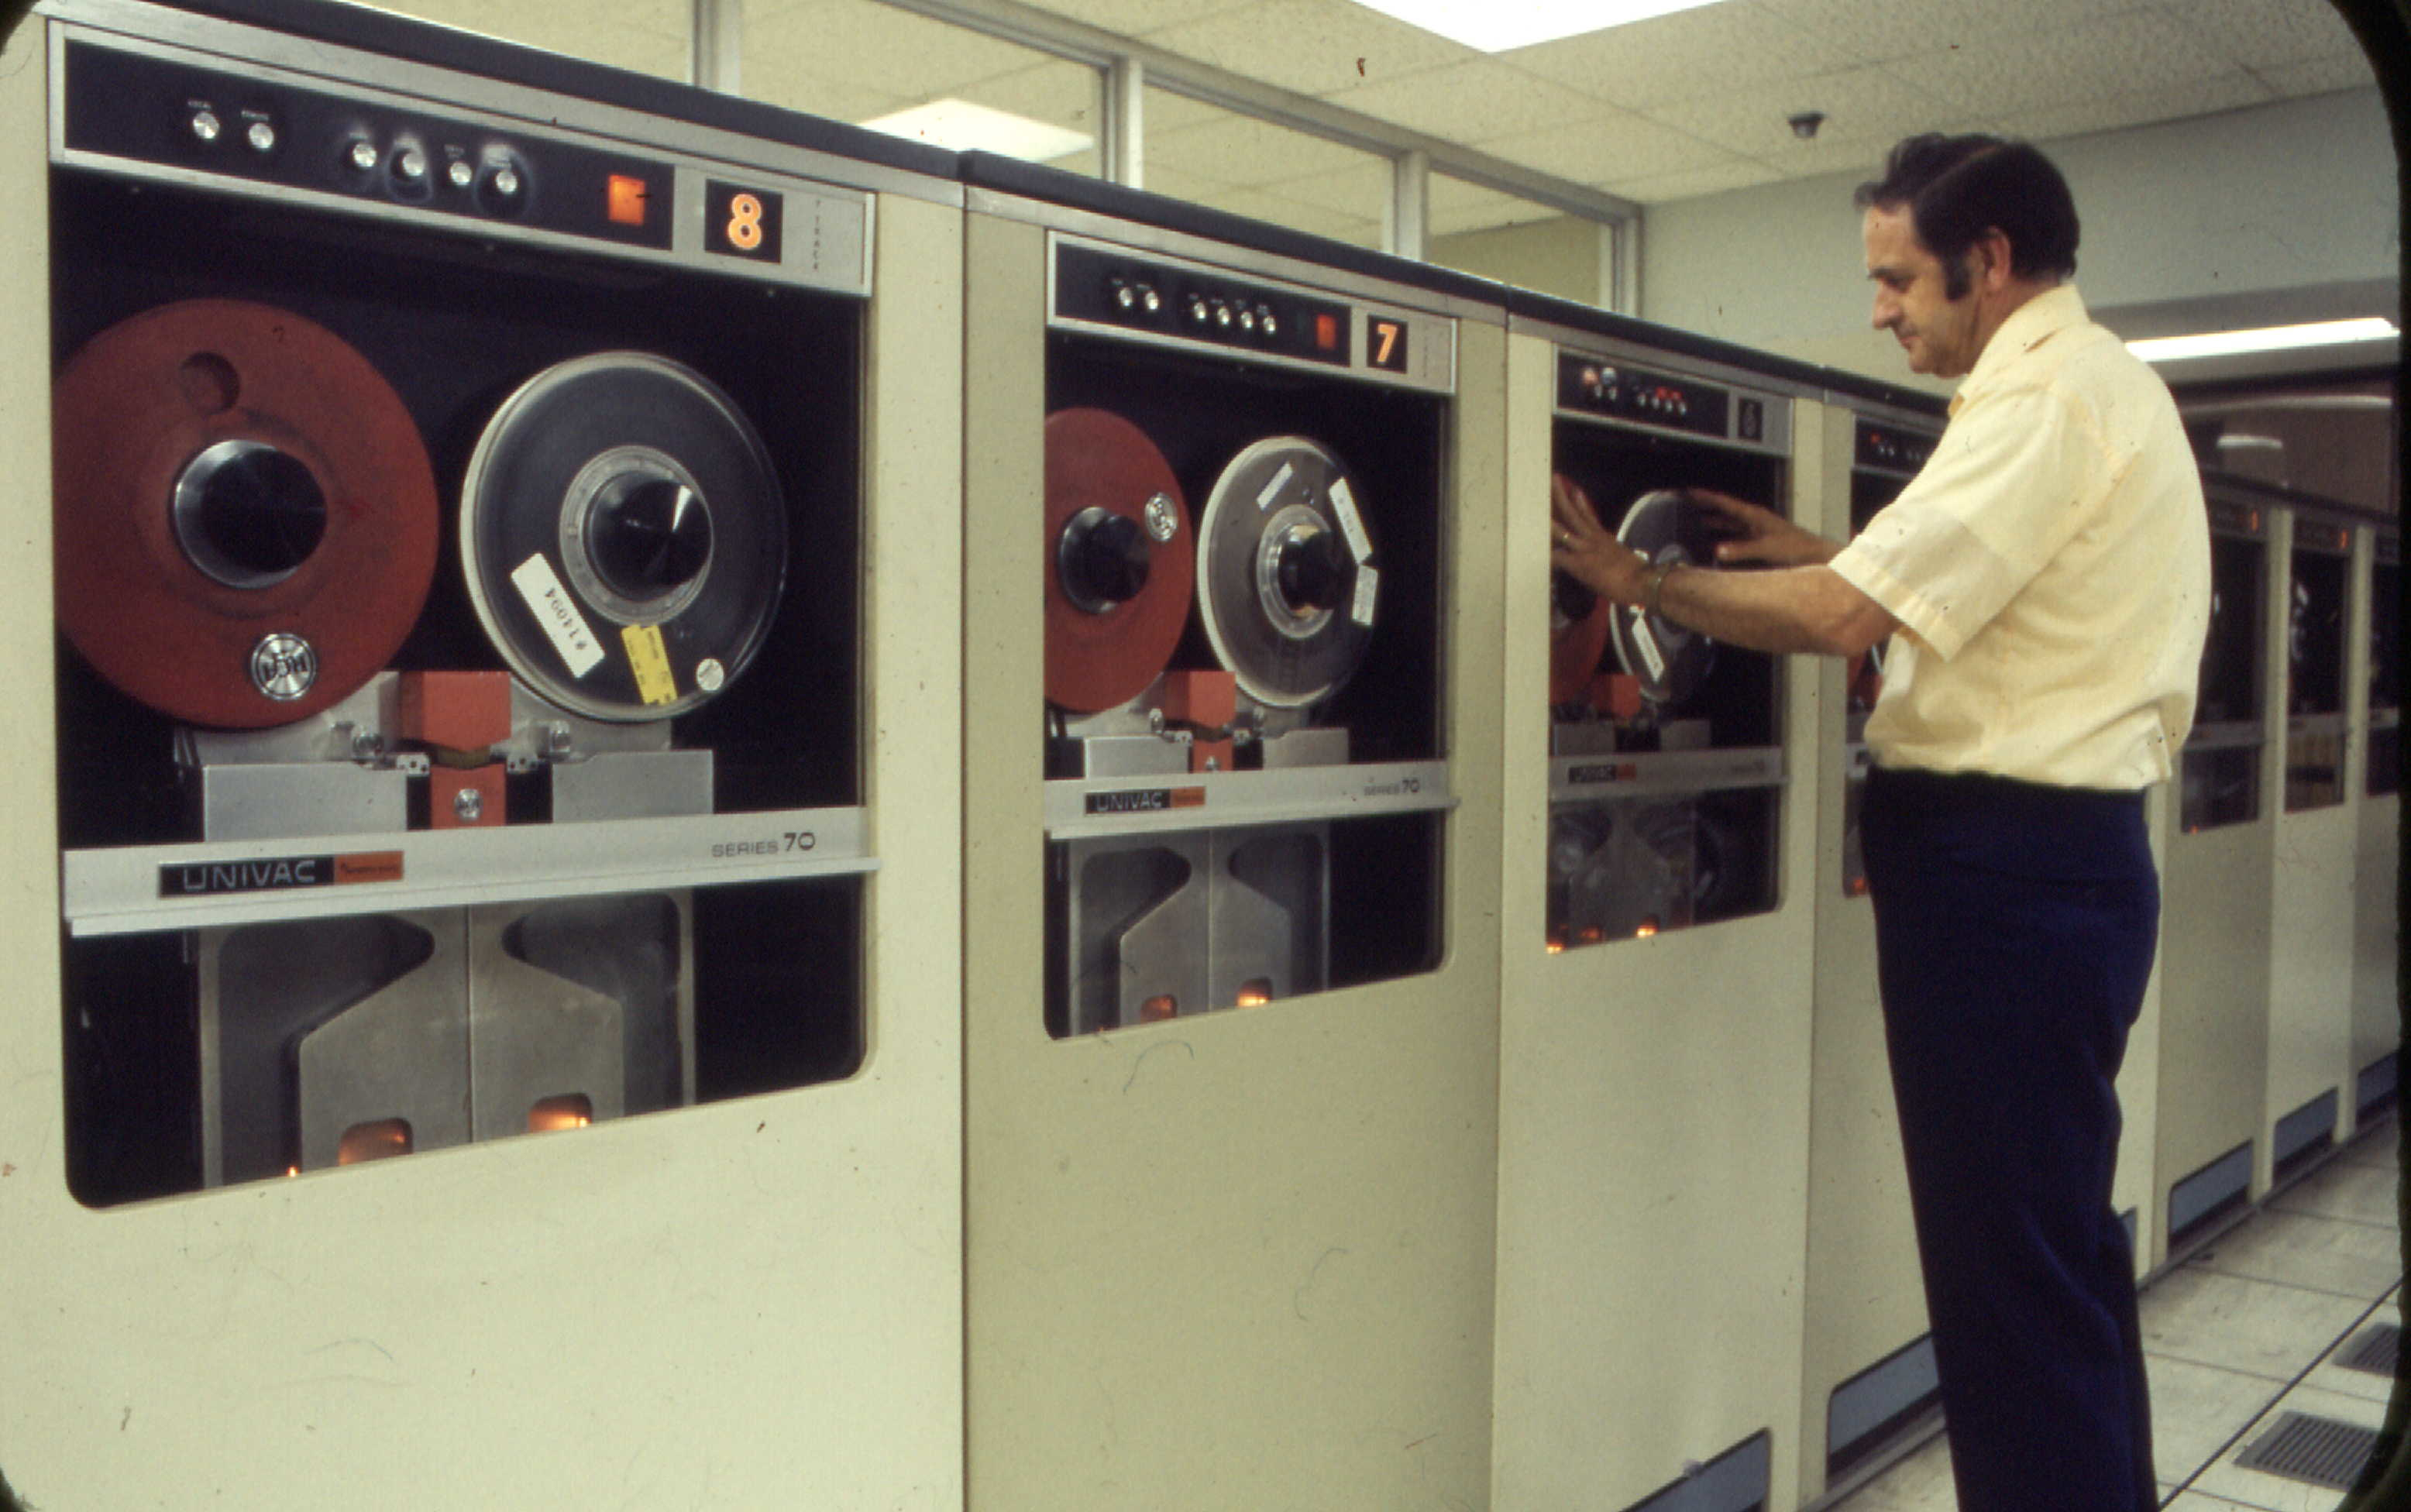
\includegraphics[width=\textwidth]{./img/file-structure-drive.png}
\end{frame}

% http://toto.lib.unca.edu/findingaids/photo/national_climatic_data_center/Machines%20&%20People/Tape%20drives%2070s.jpg

%%%%%%%%%%%%%%%%%%%%%%%%%%%%%%%%%%%%%%%%%%%%%%%%%%%%%%%%%%%%%%%%%%%%%%%%%%%%%%%%
\begin{frame}[fragile]
  \frametitle{File structure}

  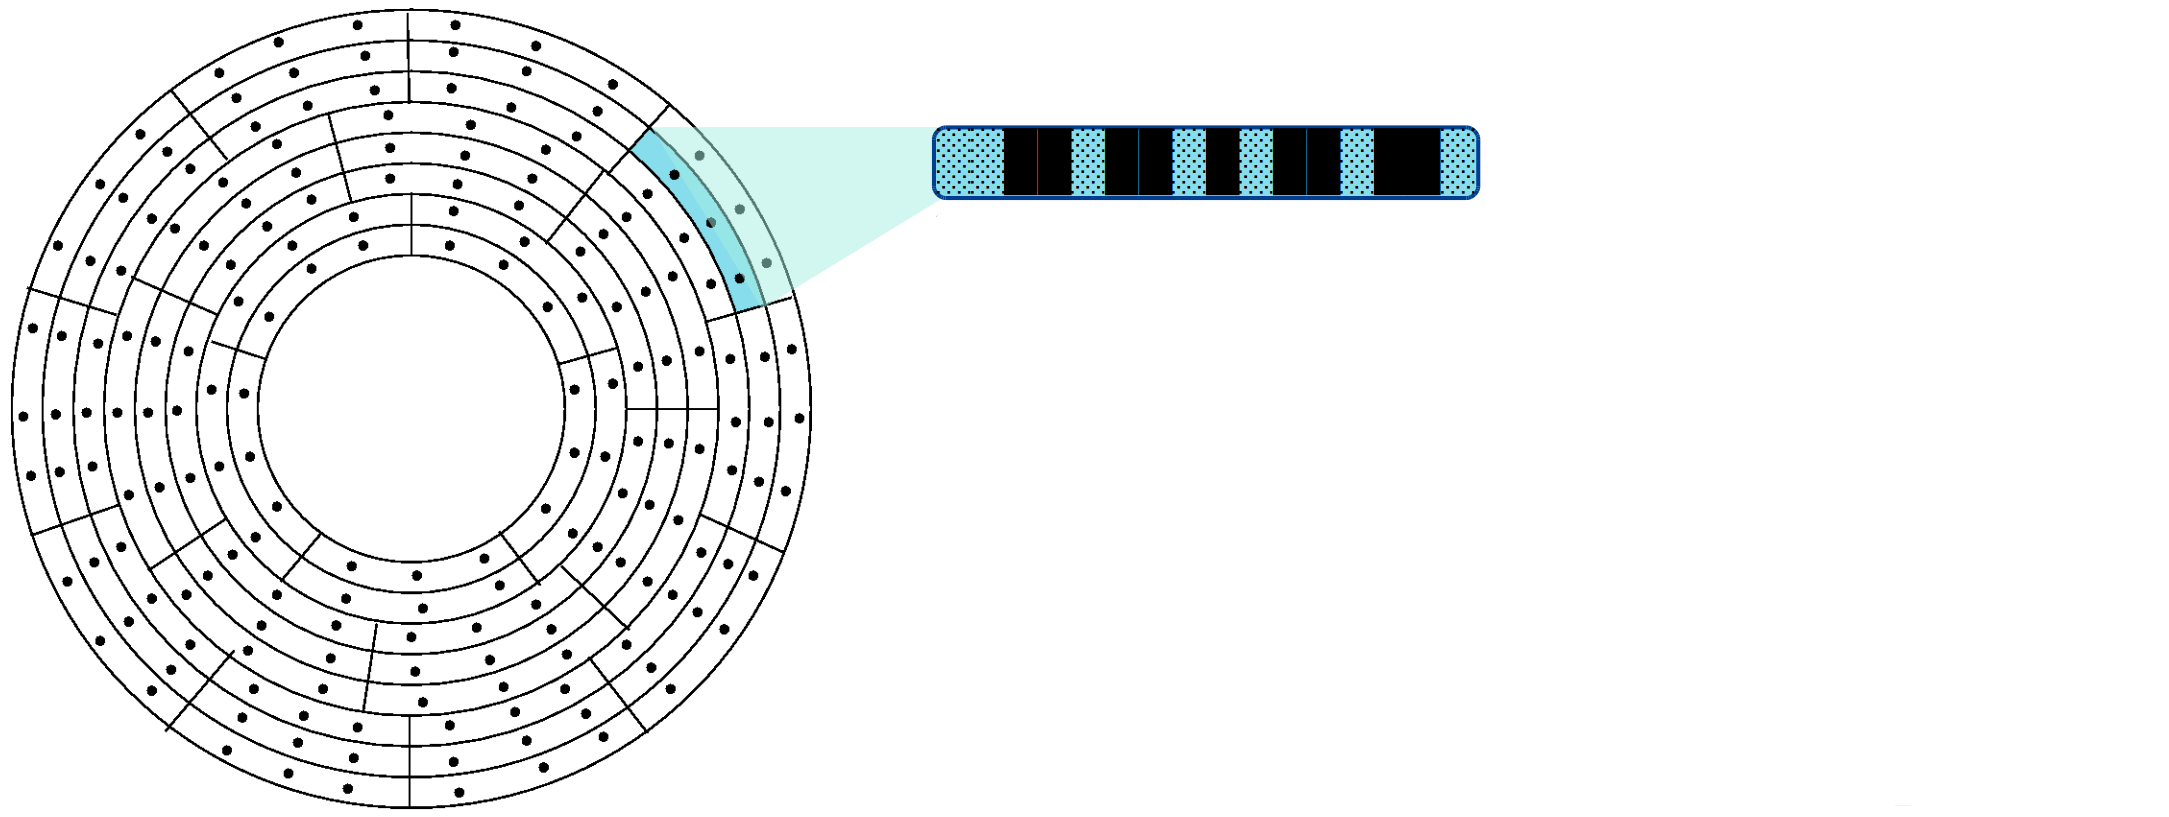
\includegraphics[width=\textwidth]{./img/file-structure-01.png}
\end{frame}

%%%%%%%%%%%%%%%%%%%%%%%%%%%%%%%%%%%%%%%%%%%%%%%%%%%%%%%%%%%%%%%%%%%%%%%%%%%%%%%%
\begin{frame}[fragile]
  \frametitle{File structure}

  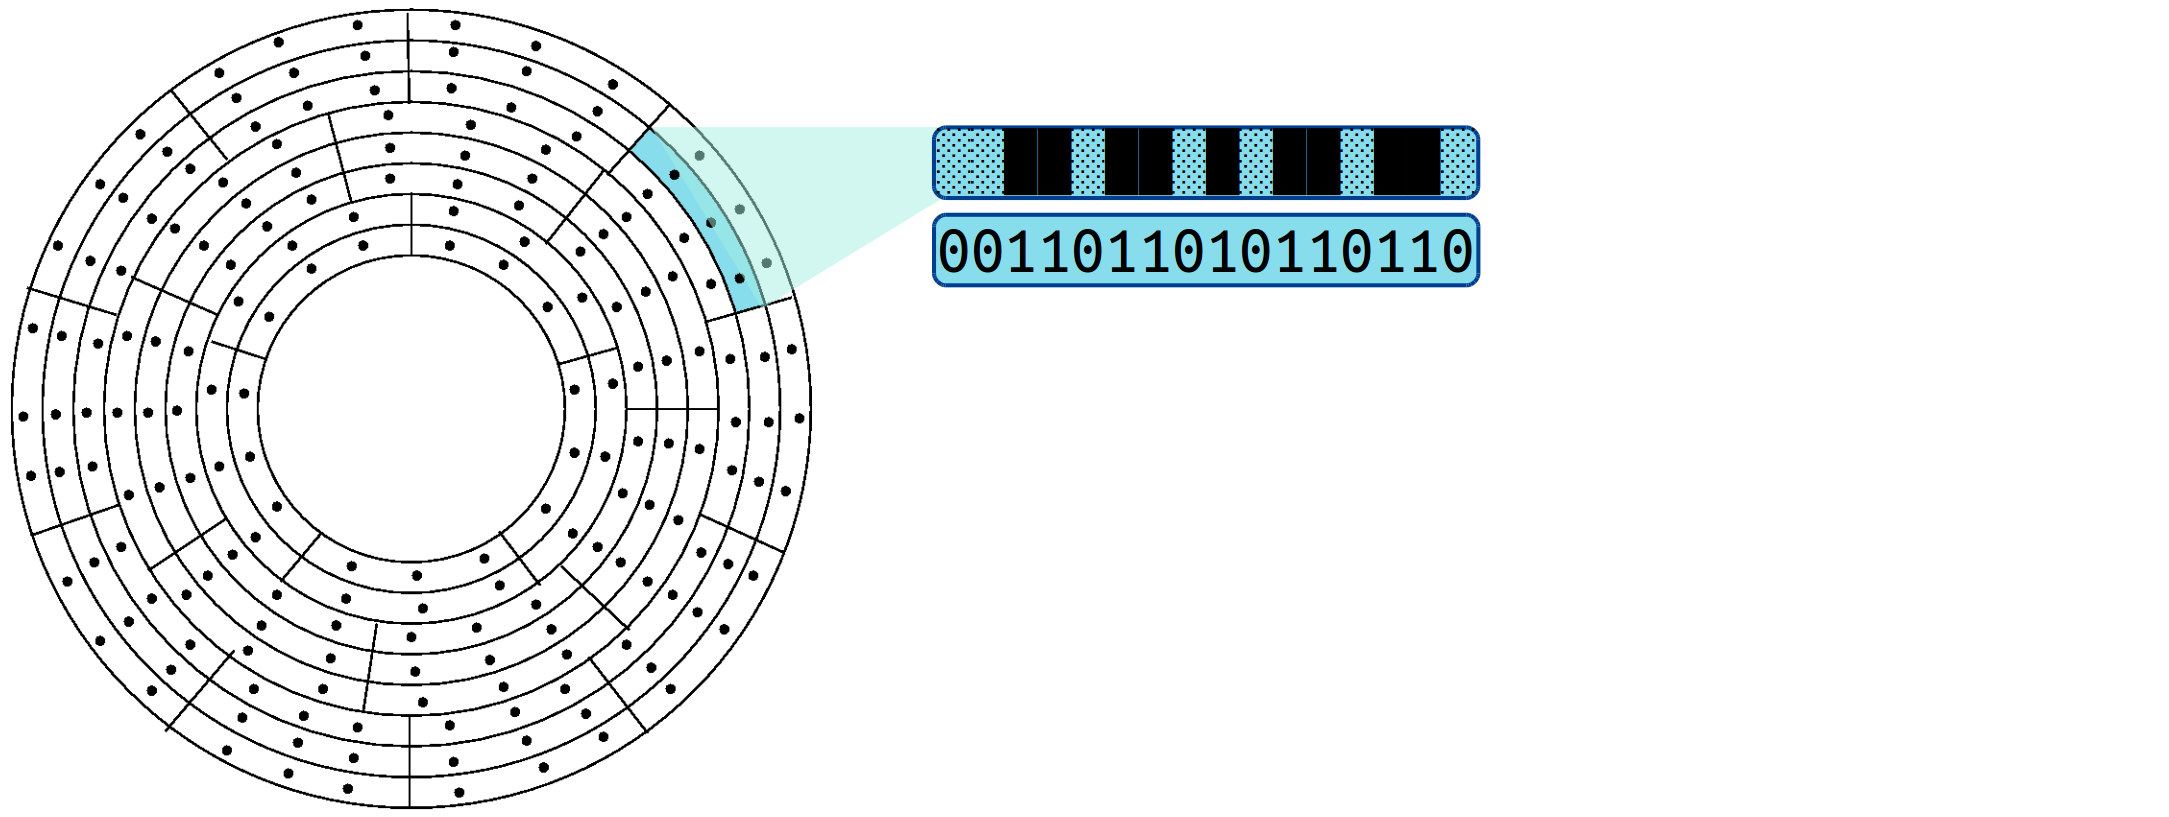
\includegraphics[width=\textwidth]{./img/file-structure-02.png}
\end{frame}

%%%%%%%%%%%%%%%%%%%%%%%%%%%%%%%%%%%%%%%%%%%%%%%%%%%%%%%%%%%%%%%%%%%%%%%%%%%%%%%%
\begin{frame}[fragile]
  \frametitle{File structure}

  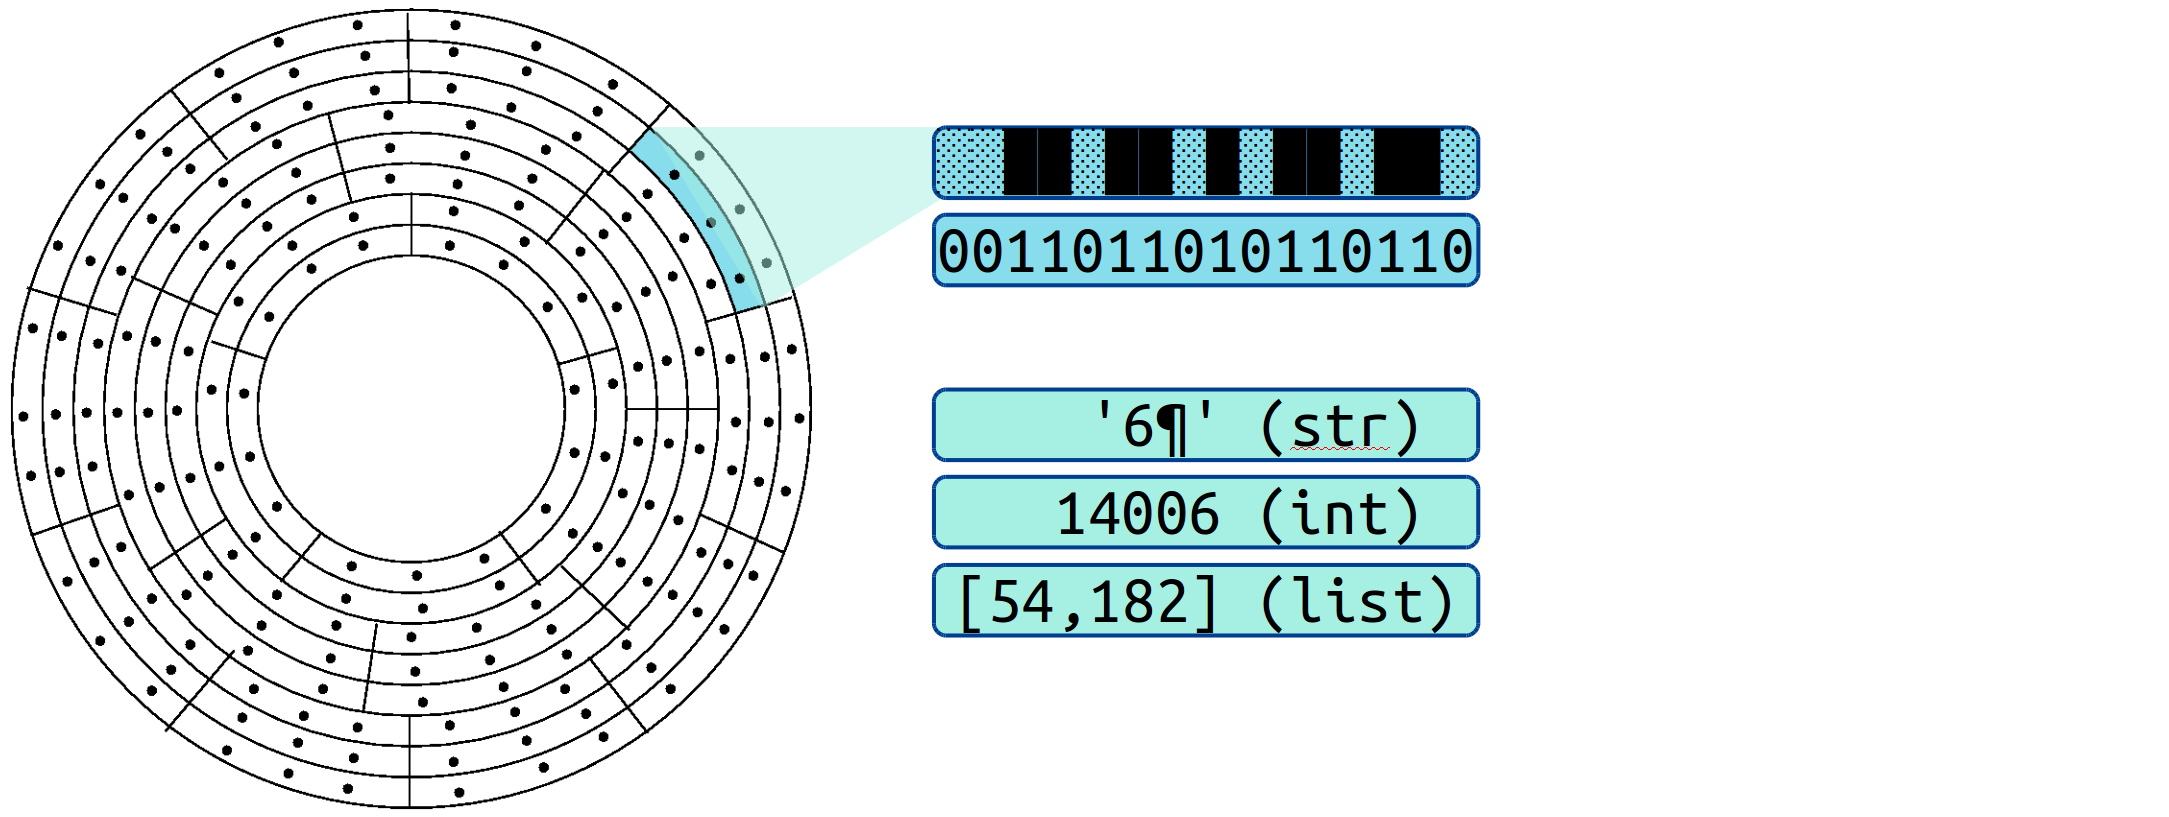
\includegraphics[width=\textwidth]{./img/file-structure-03.png}
\end{frame}

%%%%%%%%%%%%%%%%%%%%%%%%%%%%%%%%%%%%%%%%%%%%%%%%%%%%%%%%%%%%%%%%%%%%%%%%%%%%%%%%
\begin{frame}[fragile]
  \frametitle{File structure}

  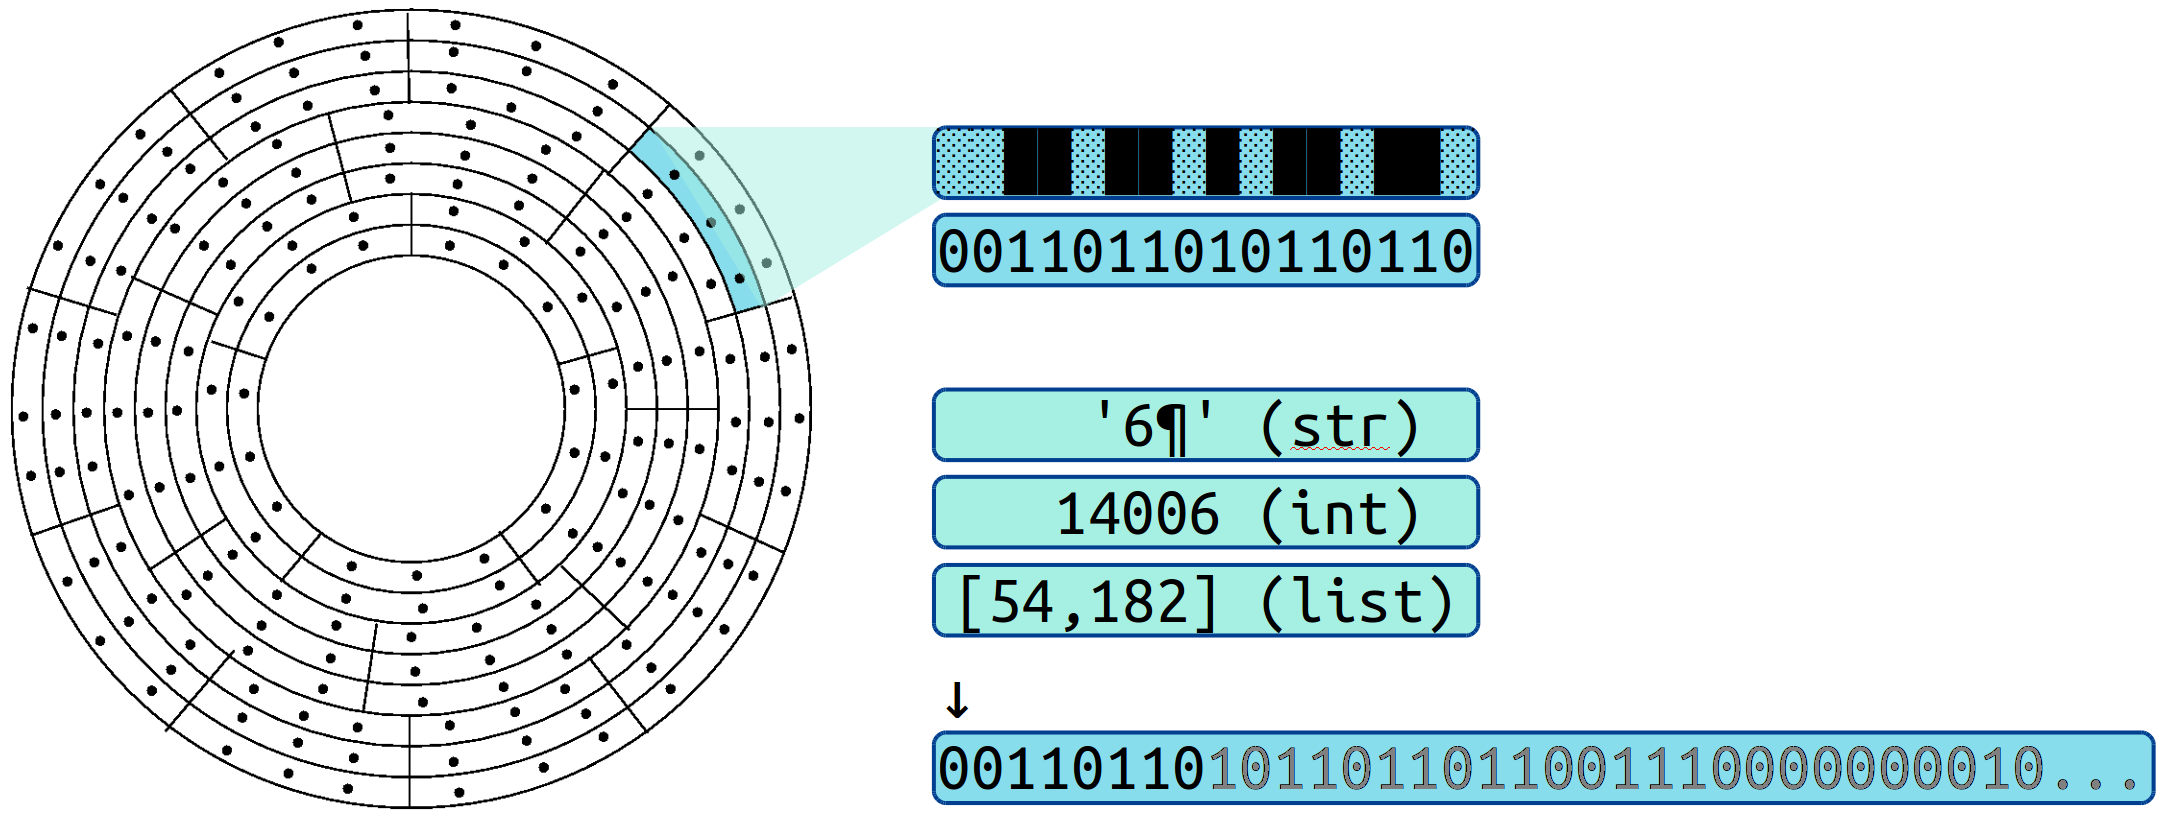
\includegraphics[width=\textwidth]{./img/file-structure-04a.png}
\end{frame}

%%%%%%%%%%%%%%%%%%%%%%%%%%%%%%%%%%%%%%%%%%%%%%%%%%%%%%%%%%%%%%%%%%%%%%%%%%%%%%%%
\begin{frame}[fragile]
  \frametitle{File structure}

  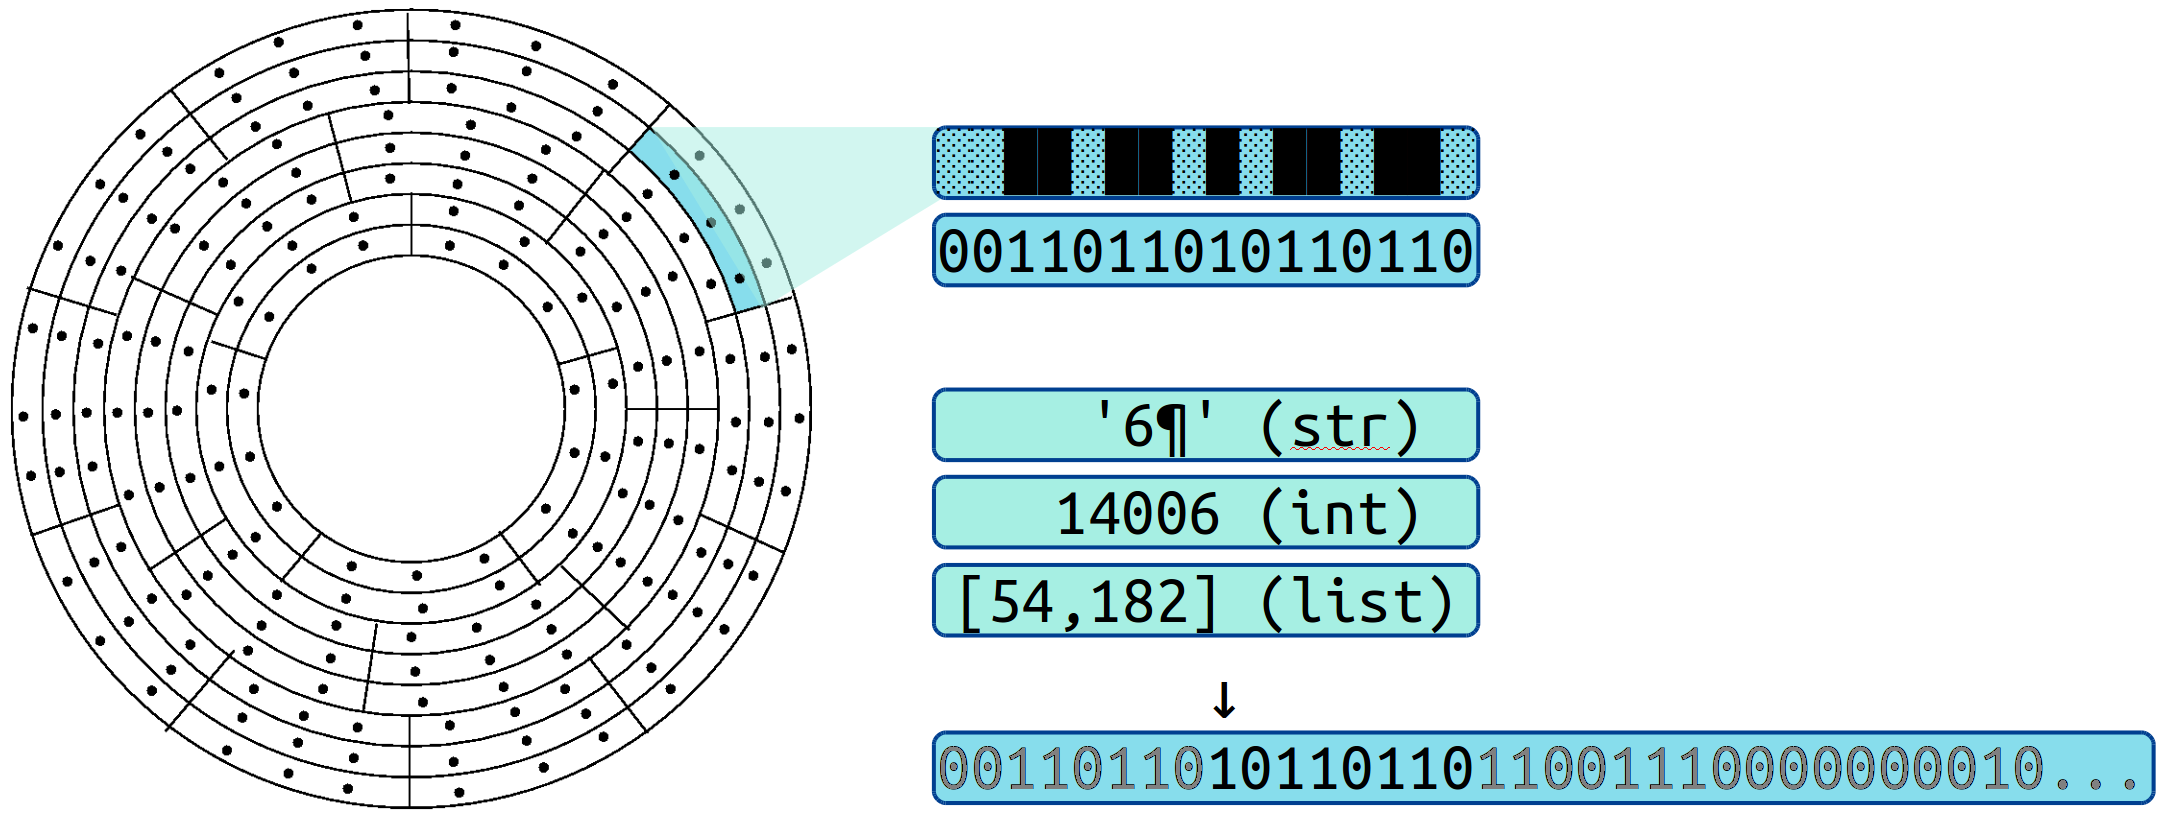
\includegraphics[width=\textwidth]{./img/file-structure-04b.png}
\end{frame}

%%%%%%%%%%%%%%%%%%%%%%%%%%%%%%%%%%%%%%%%%%%%%%%%%%%%%%%%%%%%%%%%%%%%%%%%%%%%%%%%
\begin{frame}[fragile]
  \frametitle{File structure}

  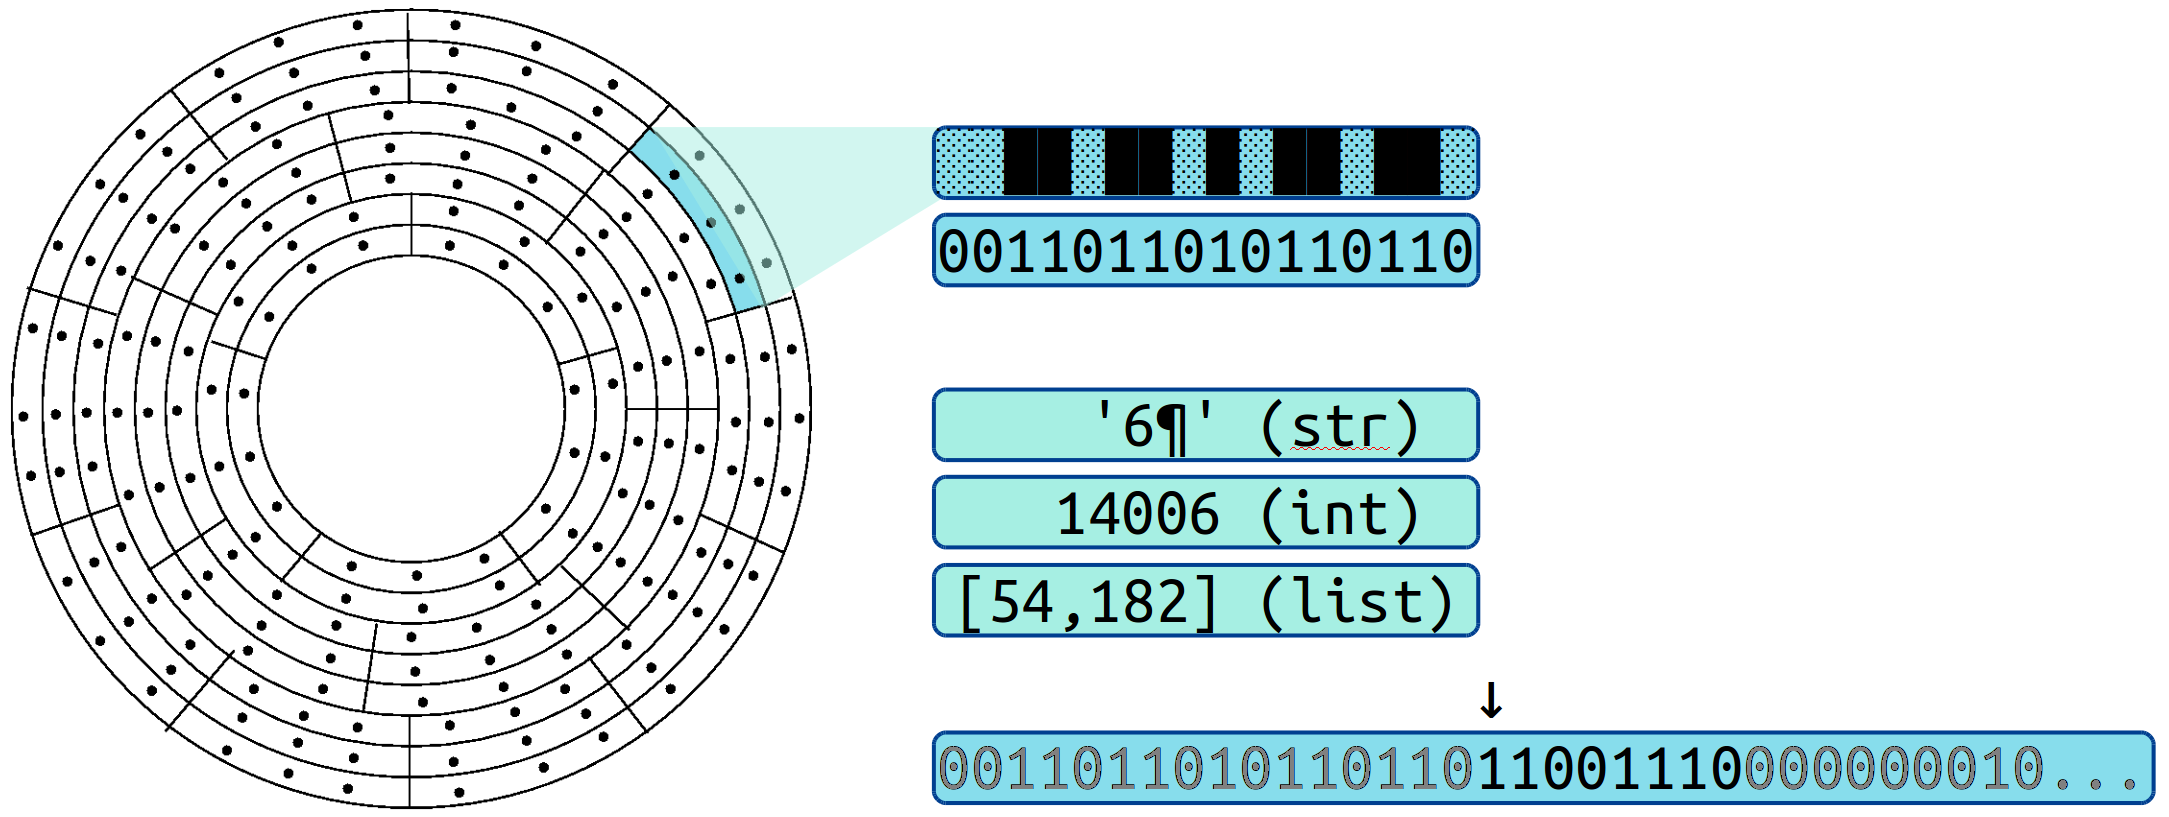
\includegraphics[width=\textwidth]{./img/file-structure-04c.png}
\end{frame}

%%%%%%%%%%%%%%%%%%%%%%%%%%%%%%%%%%%%%%%%%%%%%%%%%%%%%%%%%%%%%%%%%%%%%%%%%%%%%%%%
\begin{frame}[fragile]
  \frametitle{Files}
  \Enlarge

  \begin{itemize}
  \myitem  \texttt{file} is an iterable type created by the function \texttt{open}.
  \myitem  \texttt{open} accepts one option:  the file name as a string (for now).
  \myitem  Each item in the iterable is a string representing one line in the file.
  \end{itemize}
  \begin{semiverbatim}
myfile = open( 'wordlist.txt' )
for line in myfile:
    print( line )
  \end{semiverbatim}
\end{frame}

%%%%%%%%%%%%%%%%%%%%%%%%%%%%%%%%%%%%%%%%%%%%%%%%%%%%%%%%%%%%%%%%%%%%%%%%%%%%%%%%
\begin{frame}[fragile]
  \frametitle{Example}
  \Enlarge

  \begin{semiverbatim}
total = 0
for line in open( 'numbers.txt' ):
    total += int( line )

print( total )
  \end{semiverbatim}
\end{frame}

%%%%%%%%%%%%%%%%%%%%%%%%%%%%%%%%%%%%%%%%%%%%%%%%%%%%%%%%%%%%%%%%%%%%%%%%%%%%%%%%
\begin{frame}[fragile]
  \frametitle{Example}
  \Enlarge

  \begin{semiverbatim}
for w in open( 'words.txt' ):
    vowels = 0
    for c in w.lower():
        if c in 'aeiou':
            vowels += 1
    print( w.strip() + ' %i' % vowels )
  \end{semiverbatim}
\end{frame}

%%%%%%%%%%%%%%%%%%%%%%%%%%%%%%%%%%%%%%%%%%%%%%%%%%%%%%%%%%%%%%%%%%%%%%%%%%%%%%%%
\begin{frame}[fragile]
  \frametitle{File workflow}
  \Enlarge

  \begin{itemize}
  \myitem  If we \texttt{open} a  \texttt{file}, we should \texttt{close} it as well.
  \myitem  \texttt{close} protects the file against data loss.
  \end{itemize}
  \begin{semiverbatim}
myfile = open( 'wordlist.txt' )
for line in myfile:
    print( line )
myfile.close()  # process responsibly
  \end{semiverbatim}
\end{frame}

%%%%%%%%%%%%%%%%%%%%%%%%%%%%%%%%%%%%%%%%%%%%%%%%%%%%%%%%%%%%%%%%%%%%%%%%%%%%%%%%
\begin{frame}[fragile]
  \frametitle{File modes}
  \Enlarge

  \begin{itemize}
  \myitem  The default way of opening a \texttt{file} is to read it.
  \myitem  We can extract all of the data from the file at once with:
    \begin{itemize}
    \mysubitem  \texttt{read}, which returns a string
    \end{itemize}
  \end{itemize}
  \begin{semiverbatim}
myfile = open( 'wordlist.txt' )
mydata = myfile.read()
myfile.close()
print( mydata )
  \end{semiverbatim}
\end{frame}

%%%%%%%%%%%%%%%%%%%%%%%%%%%%%%%%%%%%%%%%%%%%%%%%%%%%%%%%%%%%%%%%%%%%%%%%%%%%%%%%
\begin{frame}[fragile]
  \frametitle{File modes}
  \Enlarge

  \begin{itemize}
  \myitem  The default way of opening a \texttt{file} is to read it.
  \myitem  We can extract all of the data from the file at once with:
    \begin{itemize}
    \mysubitem  \texttt{read}, which returns a string
    \mysubitem  \texttt{readlines}, which returns a \texttt{list} of strings
    \end{itemize}
  \end{itemize}
  \begin{semiverbatim}
myfile = open( 'wordlist.txt' )
mydata = myfile.readlines()
myfile.close()
for line in mydata:
    print( line )
  \end{semiverbatim}
\end{frame}

%%%%%%%%%%%%%%%%%%%%%%%%%%%%%%%%%%%%%%%%%%%%%%%%%%%%%%%%%%%%%%%%%%%%%%%%%%%%%%%%
\begin{frame}[fragile]
  \frametitle{File modes}
  \Enlarge

  \begin{itemize}
  \myitem  We can also \texttt{write} to a \texttt{file}, but we need to \texttt{open} it differently.
  \myitem  We can specify a file mode when we open a file:
    \begin{itemize}
    \mysubitem  \texttt{'r'} to read a \texttt{file}'s data (default)
    \mysubitem  \texttt{'w'} to write data to a \texttt{file}
    \end{itemize}
  \end{itemize}
  \begin{semiverbatim}
myfile = open( 'wordlist.txt','w' )
myfile.write( 'Hello, this is a test.' )
myfile.close()  # ultra-important now!
  \end{semiverbatim}
  \begin{itemize}
  \myitem  Other modes available but not important for 101.
  \end{itemize}
\end{frame}

%TODO: work a couple of examples

%%%%%%%%%%%%%%%%%%%%%%%%%%%%%%%%%%%%%%%%%%%%%%%%%%%%%%%%%%%%%%%%%%%%%%%%%%%%%%%%
\section{Reminders}

%%%%%%%%%%%%%%%%%%%%%%%%%%%%%%%%%%%%%%%%%%%%%%%%%%%%%%%%%%%%%%%%%%%%%%%%%%%%%%%%
\begin{frame}
  \frametitle{Reminders}
  \Enlarge

  \begin{itemize}
  \myitem  Homework \#5 is due Friday Sep.\ 30.
  \myitem  Midterm \#1 will be Monday Oct.\ 3.  (evening) \\ \textcolor{CS101GradBot}{No class on Monday, \\ Labs WILL be held all week.}
  \end{itemize}
\end{frame}

\end{document}
